\documentclass[a4paper,12pt]{article} % добавить leqno в [] для нумерации слева
\usepackage[a4paper,top=1.3cm,bottom=2cm,left=1.5cm,right=1.5cm,marginparwidth=0.75cm]{geometry}
%%% Работа с русским языком
\usepackage{cmap}					% поиск в PDF
\usepackage[warn]{mathtext} 		% русские буквы в фомулах
\usepackage[T2A]{fontenc}			% кодировка
\usepackage[utf8]{inputenc}			% кодировка исходного текста
\usepackage[english,russian]{babel}	% локализация и переносы
\usepackage{physics}
\usepackage{multirow}

%%% Нормальное размещение таблиц (писать [H] в окружении таблицы)
\usepackage{float}
\restylefloat{table}


\usepackage{graphicx}

\usepackage{wrapfig}
\usepackage{tabularx}

\usepackage{hyperref}
\usepackage[rgb]{xcolor}
\hypersetup{
	colorlinks=true,urlcolor=blue
}

%%% Дополнительная работа с математикой
\usepackage{amsmath,amsfonts,amssymb,amsthm,mathtools} % AMS
\usepackage{icomma} % "Умная" запятая: $0,2$ --- число, $0, 2$ --- перечисление

%% Номера формул
%\mathtoolsset{showonlyrefs=true} % Показывать номера только у тех формул, на которые есть \eqref{} в тексте.

%% Шрифты
\usepackage{euscript}	 % Шрифт Евклид
\usepackage{mathrsfs} % Красивый матшрифт
\usepackage{pgfplots}
\pgfplotsset{compat=1.9}

%% Свои команды
\DeclareMathOperator{\sgn}{\mathop{sgn}}

%% Перенос знаков в формулах (по Львовскому)
\newcommand*{\hm}[1]{#1\nobreak\discretionary{}
	{\hbox{$\mathsurround=0pt #1$}}{}}

\date{\today}

\begin{document}

\begin{titlepage}
	\begin{center}
		{\large МОСКОВСКИЙ ФИЗИКО-ТЕХНИЧЕСКИЙ ИНСТИТУТ (НАЦИОНАЛЬНЫЙ ИССЛЕДОВАТЕЛЬСКИЙ УНИВЕРСИТЕТ)}
	\end{center}
	\begin{center}
		{\large Физтех-школа физики и исследований им. Ландау}
	\end{center}
	
	
	\vspace{4.5cm}
	{\huge
		\begin{center}
			{\bf Отчёт о выполнении лабораторной работы 3.2.2}\\
			Резонанс напряжений
		\end{center}
	}
	\vspace{2cm}
	\begin{flushright}
		{\LARGE Автор:\\ Сенокосов Арсений Олегович \\
			\vspace{0.2cm}
			Б02-012}
	\end{flushright}
	\vspace{8cm}
	\begin{center}
		Долгопрудный\\
		\today
	\end{center}
\end{titlepage}


\section{Введение}

\textbf{Цель работы:} изучение последовательной цепи переменного тока, наблюдение резонанса напряжений.

\textbf{В работе используются:} регулировочный автотрансформатор, катушка индуктивности с выдвижным сердечником, магазин ёмкостей, реостат, резистор, амперметр, три вольтметра, ваттметр, осциллограф, универсальный мост.

\section{Теоретические сведения}

Рассмотрим электрическую цепь, состоящую из резистора $ R $ и катушки индуктивности $ L $ с импедансом $ Z_L = r_L + i \Omega L $, последовательно подключённых к внешнему источнику, ЭДС которого меняется по синусоидальному закону с частотой $ \Omega $ (рис. \ref{fig:image1}).
\begin{figure}[h]
	\center{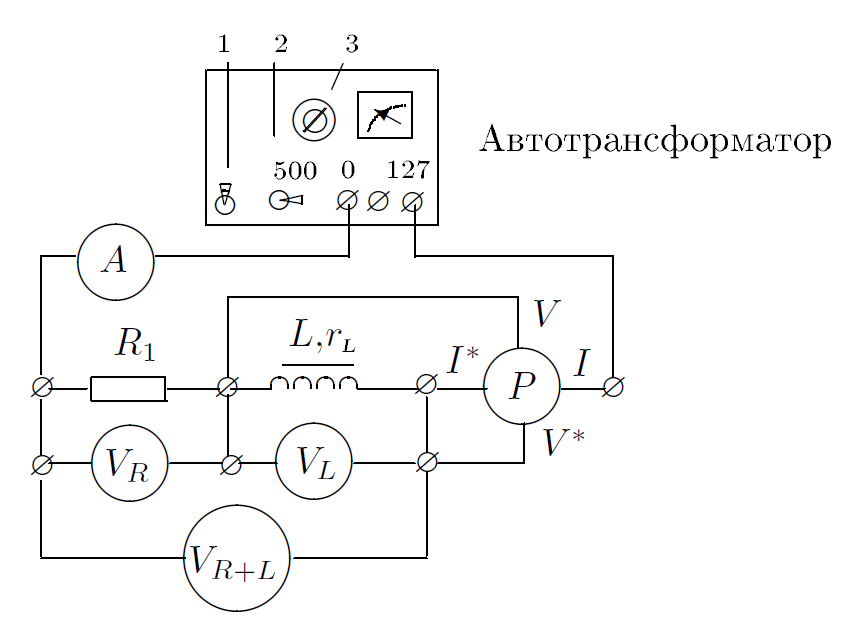
\includegraphics[scale=0.8]{Screenshot_2.png}}
	\caption{\centering Схема установки для изучения закона Ома в цепи переменного тока.}
	\label{fig:image1}
\end{figure}

Обозначим через $ U_R $ напряжение на резисторе, через $ U_L $ -- напряжение на катушке и через $ U_{R+L} $ — суммарное напряжение на катушке и на резисторе. Для этих напряжений справедливы комплексные соотношения:
\begin{equation}\label{eq:1}
{\widehat U_R} = \widehat IR, \quad {\widehat U_L} = \widehat I\left( {{r_L} + i\Omega L} \right), \quad {\widehat U_{R + L}} = \widehat I\left( {R + {r_L} + i\Omega L} \right).
\end{equation}
Напомним, что здесь $ r_L $ -- активное сопротивление катушки, которое характеризует суммарные потери энергии в катушке, в том числе потери в её ферромагнитном сердечнике.

Переходя к модулям и фазам токов и напряжений, найдём из (\ref{eq:1}):
\begin{equation}\label{eq:2}
{U_R} = I \cdot R, \quad \tg{\psi _1} = 0;
\end{equation}
\begin{equation}\label{eq:3}
{U_L} = I \cdot \sqrt {r_L^2 + {{\left( {\Omega L} \right)}^2}}, \quad \tg{\psi _2} = \frac{{\Omega L}}{{{r_L}}};
\end{equation}
\begin{equation}\label{eq:4}
{U_{R + L}} = I\sqrt {{{\left( {R + {r_L}} \right)}^2} + {{\left( {\Omega L} \right)}^2}}, \quad \tg{\psi _3} = \frac{{\Omega L}}{{R + {r_L}}}.
\end{equation}
В этих формулах $ U $ и $ I $ обозначают \textit{эффективные} значения напряжений и токов (показания приборов), как принято в электротехнике.

Измеряя с помощью трёх вольтметров значения $ U_R $, $ U_L $ и $ U_{R+L} $ и зная сопротивление резистора $ R $, нетрудно вычислить, пользуясь формулами (\ref{eq:2}), (\ref{eq:3}) и (\ref{eq:4}), силу тока в цепи, активное сопротивление катушки $ r_L $, её индуктивность $ L $, мощность $ P_L $, выделяемую на катушке, и сдвиг фаз между током и напряжением на катушке.

Рассчитаем мощность переменного тока, выделяемую в катушке. Мгновенное значение мощности равно
\begin{equation*}
P = U\left( t \right) \cdot I\left( t \right).
\end{equation*}
Средняя мощность за период $ T $ определяется формулой
\begin{equation*}
\overline P  = \frac{1}{T}\int\limits_0^T {U\left( t \right) \cdot I\left( t \right)dt}.
\end{equation*}
Полагая $ \displaystyle I\left( t \right) = I\sqrt 2 \cos \Omega t $, $ U\left( t \right) = U\sqrt 2 \cos \left( {\Omega t + \psi } \right) $, получим после интегрирования:
\begin{equation}\label{eq:5}
{P_L} = {U_L} \cdot I\cos \psi  = {I^2} \cdot {r_L}.
\end{equation}
Средняя мощность, выделяющаяся в катушке самоиндукции, определяется, таким образом, действительной частью её импеданса.

Активное сопротивление катушки $ r_L $ можно определить, если включить её в последовательный колебательный контур с известными параметрами -- сопротивлением $ R $ и ёмкостью $ C $ (рис. \ref{fig:image2}). В контуре, настроенном в резонанс на частоту $ \Omega $ внешнего источника (собственная частота контура и внешняя совпадают: $ \omega_0 = \Omega $, реактивные сопротивления индуктивности и ёмкости одинаковы:
\begin{equation}\label{eq:6}
{\omega _0}L = \frac{1}{{{\omega _0}C}}.
\end{equation}
Определив каким-либо экспериментальным способом добротность $ Q $ этого контура, можно рассчитать полное сопротивление контура $ R_{\Sigma} $ в резонансе, поскольку
\begin{equation}\label{eq:7}
Q = \frac{{{\omega _0}L}}{{{R_\Sigma }}} = \frac{1}{{{\omega _0}C{R_\Sigma }}}.
\end{equation}
Резонансное сопротивление контура $ R_{\Sigma} $, включает в себя известное со противление резистора $ R $ и активное сопротивление катушки $ r_L $:
\begin{equation}\label{eq:8}
{R_\Sigma } = R + {r_L}.
\end{equation}

\section{Экспериментальная установка}
Схема установки для исследования закона Ома в цепи переменного тока представлена на рис. \ref{fig:image1}. Цепь, состоящая из резистора $ R_1 \simeq 100 $ Ом и катушки $ L $ с выдвижным сердечником, подключена к автотрансформатору, выходное напряжение которого можно менять от $ 0 $ до $ 127 $ В. Напряжения на каждом из элементов и суммарное напряжение цепи измеряются тремя вольтметрами: $ V_R $, $ V_L $ и $ V_{R+L} $. Амперметр $ A $ измеряет ток в цени, а ваттметр $ P $ -- мощность, выделяющуюся на катушке.

Ваттметр электродинамической системы состоит из двух катушек, одна из которых вращается в магнитном поле другой, если через них течёт ток. Токовая катушка ваттметра $ II $* включается последовательно в исследуемую цепь, а катушка напряжений (потенциальная) $ VV $* -- параллельно к элементу, в котором измеряется выделяемая мощность.

Два из четырёх зажимов ваттметра помечены звёздочкой (*). Эти зажимы надо соединить вместе. Предел измерений устанавливается при помощи переключателей или штепселей, которые вставляются в соответствующие гнёзда: произведение цифр против штепселя токовой катушки $ II $* и против переключателя катушки напряжений $ VV $* определяет мощность, соответствующую отклонению стрелки на всю шкалу. Отсчёт мощности ведётся но любой из шкал, обозначенных буквой $ P $.

\begin{figure}[h]
	\center{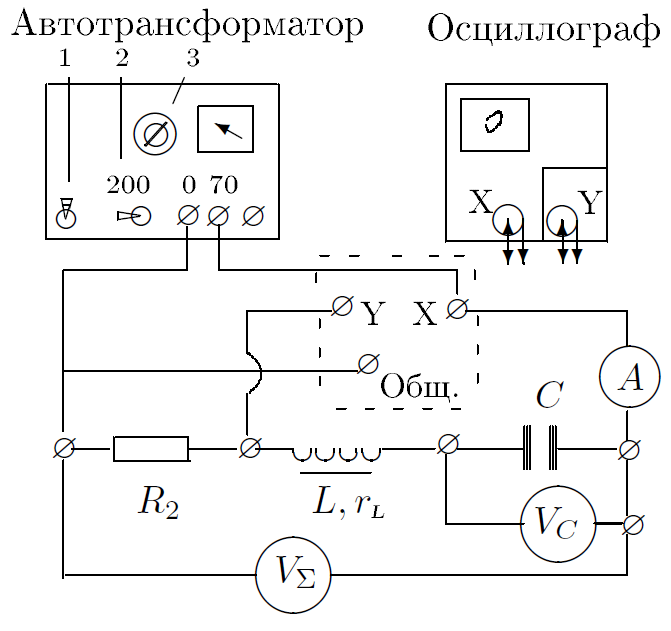
\includegraphics[scale=0.8]{Screenshot_3.png}}
	\caption{\centering Схема установки для наблюдения резонанса напряжений.}
	\label{fig:image2}
\end{figure}

Схема установки для изучения резонанса напряжений изображена на рис. \ref{fig:image2}. Последовательно соединены резистор $ R_2 \approx 5 $ Ом, катушка $ L $ и магазин ёмкостей $ C $. Амперметр $ A $ измеряет ток в цепи, вольтметр $ V_C $ — напряжение на ёмкости, вольтметр $ V_{\Sigma} $ -- суммарное напряжение на контуре. Резонанс можно зафиксировать с помощью осциллографа, если подать на вход $ X $ напряжение с контура, а на вход $ Y $ -- напряжение с резистора $ R_2 $, пропорциональное току в цепи. В общем случае на экране виден эллипс. При резонансе эллипс вырождается в прямую линию.
Резонансные напряжения на контуре $ U_{\Sigma,\text{ рез}} $ и на ёмкости $ U_{C,\text{ рез}} $ равны соответственно
\begin{equation}\label{eq:9}
U_{\Sigma,\text{ рез}} = I_{\text{рез}}R_{\Sigma}, \quad U_{C,\text{ рез}} = \dfrac{I_{\text{рез}}}{\Omega C}.
\end{equation}
Сравнивая (\ref{eq:7}) и (\ref{eq:9}), получим
\begin{equation}\label{eq:10}
Q = \dfrac{U_{C,\text{ рез}}}{U_{\Sigma,\text{ рез}}}, \quad {\sigma _Q} = Q\sqrt {{{\left( {\frac{{{\sigma_{U_{C,\text{ рез}}}}}}{U_{C,\text{ рез}}}} \right)}^2} + {{\left( {\frac{{{\sigma_{U_{\Sigma,\text{ рез}}}}}}{U_{\Sigma,\text{ рез}}}} \right)}^2}} .
\end{equation}
Формула (\ref{eq:10}) показывает, что добротность контура может быть найдена по измеренным значениям напряжений на контуре и на конденсаторе при резонансе. Зная добротность контура и ёмкость $ C $, можно рассчитать $ R_{\Sigma} $, по формуле (\ref{eq:7}), а затем определить $ r_L $.

\section{Ход работы}
\subsection{Закон Ома в цепи переменного тока}

Соберём цепь согласно рисунку \ref{fig:image1}. Реостат подключим без движка $ R_1 = (98,00 \pm 0,01) $ Ом. Указатель положения сердечника катушки $ L $ установим на отметку $ x = 5 $ мм. Перемещая сердечник шагами по 2 мм, снимем зависимости тока $ I $, напряжений $ U_R $, $ U_L $, $ U_{R+L} $ и мощности от координаты сердечника $ x $. Полученные результаты занесём в таблицу \ref{tab:1}.

% Please add the following required packages to your document preamble:
% \usepackage[normalem]{ulem}
% \useunder{\uline}{\ul}{}
\begin{table}[H]
	\centering
	\begin{tabular}{|c|c|c|c|c|c|}
		\hline
		$ x $, мм  & $ I $, А    & $ U_R $, В & $ U_L $, В  & $ U_{R+L} $, В & $ P_L $, Вт   \\ \hline
		5  & 0,53 & 42 & 123 & 104 & 15,5 \\ \hline
		7  & 0,59 & 49 & 121 & 100 & 14,8 \\ \hline
		9  & 0,65 & 55 & 121 & 95  & 14,3 \\ \hline
		11 & 0,69 & 59 & 119 & 92  & 14,0 \\ \hline
		13 & 0,73 & 62 & 118 & 88  & 13,3 \\ \hline
		15 & 0,75 & 65 & 117 & 86  & 13,0 \\ \hline
		17 & 0,78 & 67 & 116 & 83  & 12,8 \\ \hline
		20 & 0,80 & 70 & 116 & 80  & 12,3 \\ \hline
		22 & 0,83 & 72 & 115 & 77  & 12,0 \\ \hline
		24 & 0,85 & 73 & 114 & 76  & 11,8 \\ \hline
		26 & 0,88 & 74 & 114 & 74  & 11,8 \\ \hline
		28 & 0,88 & 76 & 114 & 72  & 11,5 \\ \hline
		30 & 0,90 & 77 & 113 & 70  & 11,3 \\ \hline
		32 & 0,90 & 77 & 113 & 69  & 11,3 \\ \hline
		34 & 0,90 & 78 & 112 & 67  & 11,3 \\ \hline
		36 & 0,90 & 79 & 112 & 66  & 11,0 \\ \hline
		38 & 0,93 & 80 & 112 & 65  & 11,0 \\ \hline
		40 & 0,93 & 81 & 112 & 64  & 11,0 \\ \hline
	\end{tabular}
	\caption{Результаты измерений}
	\label{tab:1}
\end{table}

Измерения производились со следующими погрешностями: $ \sigma_x = 0,5 $ мм, $ \sigma_I = 0,025 $ А, $ \sigma_{P_L} = 0,125 $ Вт, $ \sigma_U = 0,5 $ В.

По результатам измерений $ P_L $ и $ I $ вычислим значения $ r_L $ по формуле \eqref{eq:5}, а затем определим $ L $ по формуле \eqref{eq:3}. Частота сети $ \nu_0 = 50 $ Гц.

Т.к. $ {P_L} = {I^2} \cdot {r_L} $, то
\begin{equation}\label{eq:11}
{\sigma _{{r_L}}} = {r_L}\sqrt {{{\left( {\frac{{{\sigma _{{P_L}}}}}{{{P_L}}}} \right)}^2} + 4{{\left( {\frac{{{\sigma _I}}}{I}} \right)}^2}}.
\end{equation}

Из \eqref{eq:3} получаем $ \displaystyle L = \frac{{\sqrt {{{\left( {\frac{{{U_L}}}{I}} \right)}^2} - r_L^2} }}{\Omega } $, где $ \Omega = 2 \pi \nu_0 $.

Для вывода формулы погрешности:
\begin{equation*}
{\sigma _{r_L^2}} = 2{r_L}{\sigma _{{r_L}}}, \quad {\sigma _{U_L^2}} = 2{U_L}{\sigma _{{U_L}}}, \quad {\sigma _{{I^2}}} = 2I{\sigma _I},
\end{equation*}

\begin{equation*}
{\sigma _{\frac{{U_L^2}}{{{I^2}}}}} = \frac{{U_L^2}}{{{I^2}}}\left( {\frac{{{\sigma _{U_L^2}}}}{{U_L^2}} + \frac{{{\sigma _{{I^2}}}}}{{{I^2}}}} \right), \quad {\sigma _{\left( {\frac{{U_L^2}}{{{I^2}}} - r_L^2} \right)}} = \frac{{U_L^2}}{{{I^2}}}\left( {\frac{{{\sigma _{U_L^2}}}}{{U_L^2}} + \frac{{{\sigma _{{I^2}}}}}{{{I^2}}}} \right) + 2{r_L}{\sigma _{{r_L}}},
\end{equation*}

И для $ \sigma_L $ получаем:
\begin{equation}\label{eq:12}
{\sigma _L} = \frac{L}{2}\frac{{{\sigma _{\left( {\frac{{U_L^2}}{{{I^2}}} - r_L^2} \right)}}}}{{\frac{{U_L^2}}{{{I^2}}} - r_L^2}} = \frac{L}{2}\frac{{\frac{{U_L^2}}{{{I^2}}}\left( {\frac{{{\sigma _{U_L^2}}}}{{U_L^2}} + \frac{{{\sigma _{{I^2}}}}}{{{I^2}}}} \right) + 2{r_L}{\sigma _{{r_L}}}}}{{\frac{{U_L^2}}{{{I^2}}} - r_L^2}} = L\frac{{{U_L}{\sigma _{{U_L}}} + \frac{{U_L^2{\sigma _I}}}{I} + {I^2}{r_L}{\sigma _{{r_L}}}}}{{U_L^2 - r_L^2{I^2}}}.
\end{equation}

Результаты вычислений величин и их погрешностей занесём в таблицу \ref{tab:2}.

\begin{table}[H]
	\centering
	\begin{tabular}{|c|c|c|c|c|c|c|c|}
		\hline
		$ x $, мм & $ I $, А & $ U_L $, В & $ P_L $, Вт & $ r_L $, Ом & $\sigma_{{r_L}}$,   Ом & $ L $, Гн & $\sigma_L$, Гн \\ \hline
		5         & 0,53     & 123        & 15,5        & 56,24       & 5,37                   & 0,72      & 0,04           \\ \hline
		7         & 0,59     & 121        & 14,8        & 42,73       & 3,65                   & 0,64      & 0,03           \\ \hline
		9         & 0,65     & 121        & 14,3        & 33,73       & 2,61                   & 0,58      & 0,03           \\ \hline
		11        & 0,69     & 119        & 14,0        & 29,62       & 2,17                   & 0,54      & 0,02           \\ \hline
		13        & 0,73     & 118        & 13,3        & 25,21       & 1,75                   & 0,51      & 0,02           \\ \hline
		15        & 0,75     & 117        & 13,0        & 23,11       & 1,56                   & 0,49      & 0,02           \\ \hline
		17        & 0,78     & 116        & 12,8        & 21,23       & 1,39                   & 0,47      & 0,02           \\ \hline
		20        & 0,80     & 116        & 12,3        & 19,14       & 1,21                   & 0,46      & 0,02           \\ \hline
		22        & 0,83     & 115        & 12,0        & 17,63       & 1,08                   & 0,44      & 0,02           \\ \hline
		24        & 0,85     & 114        & 11,8        & 16,26       & 0,97                   & 0,42      & 0,01           \\ \hline
		26        & 0,88     & 114        & 11,8        & 15,35       & 0,89                   & 0,41      & 0,01           \\ \hline
		28        & 0,88     & 114        & 11,5        & 15,02       & 0,87                   & 0,41      & 0,01           \\ \hline
		30        & 0,90     & 113        & 11,3        & 13,89       & 0,79                   & 0,40      & 0,01           \\ \hline
		32        & 0,90     & 113        & 11,3        & 13,89       & 0,79                   & 0,40      & 0,01           \\ \hline
		34        & 0,90     & 112        & 11,3        & 13,89       & 0,79                   & 0,39      & 0,01           \\ \hline
		36        & 0,90     & 112        & 11,0        & 13,58       & 0,77                   & 0,39      & 0,01           \\ \hline
		38        & 0,93     & 112        & 11,0        & 12,86       & 0,71                   & 0,38      & 0,01           \\ \hline
		40        & 0,93     & 112        & 11,0        & 12,86       & 0,71                   & 0,38      & 0,01           \\ \hline
	\end{tabular}
	\caption{Результаты вычислений}
	\label{tab:2}
\end{table}

По полученным данным построим на одном графике зависимости $ L $ и $ r_L $ от положения сердечника и определим по ним значения $ L $ и $ r_L $, соответствующие резонансному ($ x=17 $ мм) положению сердечника.

\begin{center}
	\begin{tikzpicture}
	\begin{axis}[
	title={Графики №1 зависимостей $ L $ и $ r_L $ от положения сердечника $ x $},
	xlabel={Положение сердечника $ x $, мм},
	ylabel={Индуктивность катушки $ L $, Гн},
	legend pos=north west,
	xmajorgrids=true,
	ymajorgrids=true,
	ymin=0.1,
	ymax=0.75,
	xmin=4,
	xmax=41,
	grid style=dashed,
	width = 450,
	height = 250,
	]
	\addplot+ [only marks,
	error bars/.cd,
	x dir=both, x explicit,
	y dir=both, y explicit,
	] table [x = x, y = y, x error = dx, y error = dy,] {
		x	dx	y		dy
		5.0000000	0.5000000	0.7243198	0.0439571
		7.0000000	0.5000000	0.6416407	0.0337719
		9.0000000	0.5000000	0.5805436	0.0271230
		11.0000000	0.5000000	0.5431139	0.0238967
		13.0000000	0.5000000	0.5120849	0.0211913
		15.0000000	0.5000000	0.4913330	0.0196348
		17.0000000	0.5000000	0.4718613	0.0182415
		20.0000000	0.5000000	0.4577424	0.0170802
		22.0000000	0.5000000	0.4403645	0.0159473
		24.0000000	0.5000000	0.4239745	0.0149214
		26.0000000	0.5000000	0.4120340	0.0141076
		28.0000000	0.5000000	0.4121560	0.0140895
		30.0000000	0.5000000	0.3974045	0.0132349
		32.0000000	0.5000000	0.3974045	0.0132349
		34.0000000	0.5000000	0.3938438	0.0131400
		36.0000000	0.5000000	0.3939530	0.0131242
		38.0000000	0.5000000	0.3834288	0.0124538
		40.0000000	0.5000000	0.3834288	0.0124538
		
	}; \label{plot_one}
	\addplot [blue, domain=4:41] {0.37593 + 0.53209*exp(-0.10069*x)}; \label{plot_two}
	\end{axis}
	\begin{axis}[
	ylabel={Активное сопротивление $ r_L $, Ом},
	legend pos=north east,
	axis y line*=right,
	axis x line=none,
	xmajorgrids=true,
	ymajorgrids=true,
	ymin=10,
	ymax=70,
	xmin=4,
	xmax=41,
	width = 450,
	height = 250,
	grid style=dashed,
	]
	\addlegendimage{/pgfplots/refstyle=plot_one}\addlegendentry{Индуктивность $ L $};
	\addlegendimage{/pgfplots/refstyle=plot_two}\addlegendentry{Аппроксимация $ L $};
	\addplot+ [only marks, mark=o, red,
	error bars/.cd,
	x dir=both, x explicit,
	y dir=both, y explicit,
	] table [x = x, y = y, x error = dx, y error = dy,] {
		x	dx	y		dy
		5.0000000	0.5000000	56.2358277	5.3749600
		7.0000000	0.5000000	42.7342689	3.6549456
		9.0000000	0.5000000	33.7278107	2.6112616
		11.0000000	0.5000000	29.6198347	2.1703429
		13.0000000	0.5000000	25.2080856	1.7546787
		15.0000000	0.5000000	23.1111111	1.5566839
		17.0000000	0.5000000	21.2278876	1.3852637
		20.0000000	0.5000000	19.1406250	1.2121281
		22.0000000	0.5000000	17.6308540	1.0842046
		24.0000000	0.5000000	16.2629758	0.9721643
		26.0000000	0.5000000	15.3469388	0.8920360
		28.0000000	0.5000000	15.0204082	0.8736990
		30.0000000	0.5000000	13.8888889	0.7868857
		32.0000000	0.5000000	13.8888889	0.7868857
		34.0000000	0.5000000	13.8888889	0.7868857
		36.0000000	0.5000000	13.5802469	0.7700793
		38.0000000	0.5000000	12.8560993	0.7101145
		40.0000000	0.5000000	12.8560993	0.7101145
		
	}; \addlegendentry{Сопротивление $ r_L $};
	\addplot [red, domain=4:41, dotted, ultra thick] {12.60392 + 70.5266 * exp(-0.12511*x)}; \addlegendentry{Аппроксимация $ r_L $};
	\end{axis}
	\end{tikzpicture}
\end{center}

Аппроксимируем полученные зависимости выражениями вида $ x(y) = y_0 + A \exp(R_0 y) $ используя метод $ \chi^2 $ и программу OriginPro 2021. Результаты аппроксимации занесём в таблицу \ref{tab:3}

\begin{table}[H]
	\centering
	\begin{tabular}{|c|c|c|c|c|c|c|}
		\hline
		& $ y_0 $       & $ \sigma_{y_0} $      & $ A $       & $ \sigma_A $       & $ R_0 $       & $ \sigma_{R_0} $      \\ \hline
		$ L $    & 0,375 Гн  & 0,004 Гн & 0,532 Гн & 0,024 Гн & -0,101 мм$ ^{-1} $ & 0,005 мм$ ^{-1} $  \\ \hline
		$ r_L $ & 12,6 Ом & 0,3 Ом & 70,5 Ом & 4,6 Ом & -0,125 мм$ ^{-1} $ & 0,006 мм$ ^{-1} $ \\ \hline
	\end{tabular}
	\caption{Данные аппроксимации}
	\label{tab:3}
\end{table}

\subsection{Резонанс напряжений}

\subsubsection{Проведение измерений}

Соберём схему согласно рис. \ref{fig:image2}. При помощи этой схемы запишем параметры контура в резонансе. Постоянное сопротивлением в цепи \underline{$ R_2 = 5,600 \pm 0,005 $ Ом}.

Резонансный ток \underline{$ I_{\text{рез}} = 2,2 \pm 0,01 $ А} и резонансные напряжения на ёмкости -- \\
\underline{$ U_{C, \text{ рез}} = 250 \pm 5 $ В} и на контуре  -- \underline{$ U_{\Sigma, \text{ рез}} = 33,5 \pm 1,5 $ В}. По формуле \eqref{eq:10} оценим добротность контура: \underline{$ Q = 7,46 \pm 0,27 $}.

Резонансное значение ёмкости \underline{$ C = 28,1 \pm 1,4 $ мкФ}, координата положения сердечника при резонансе: \underline{$ x = 17,0 \pm 0,5 $ мм}.

Таже при помощи мультиметра и RLC-метра измерим и запишем оммическое и индуктивное сопротивление катушки и её индуктивность: \underline{$ R_{\text{кат}} = 4,900 \pm 0,005 $ Ом$ L = 312,780 \pm 0,005 $ мГн,}
\\ \underline{$ r_L = 9,530 \pm 0,005 $ Ом}.

\subsubsection{Метод векторных диаграмм}

Для резонансного положения сердечника построим векторную диаграмму напряжений (рис. \ref{fig:image3}): треугольник по трём сторонам при горизонтальном расположении $ U_R $.

\begin{figure}[h]
	\center{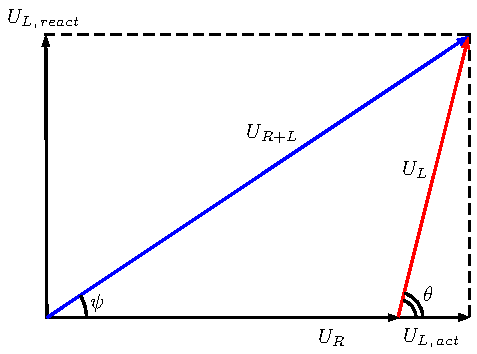
\includegraphics[scale=1]{vecd.pdf}}
	\caption{\centering Векторная диаграмма}
	\label{fig:image3}
\end{figure}

Из получившегося треугольника найдём $ U_{L,\text{ акт}} $ и $ U_{L,\text{ реакт}} $:
\begin{equation*}
\cos \psi  = \frac{{U_R^2 + U_{L + R}^2 - U_L^2}}{{2{U_R}{U_{L + R}}}}, \quad U_{L,\text{ акт}} = {U_{L + R}}\cos \psi  - {U_R}, \quad {U_{L,\text{ реакт}}} = {U_L}\sin \psi  = {U_L}\sqrt {1 - {{\cos }^2}\psi },
\end{equation*}

Получим значения:
\begin{equation}\label{eq:14t}
\underline{\cos \psi  = 0,73 \pm 0,15, \quad {U_{L,\text{ акт}}} = 14,25 \pm 17,31 \text{ В}, \quad {U_{L,\text{ реакт}}} = 55,68 \pm 11,44 \text{ В}.}
\end{equation}

Зная активное и реактивное напряжения, найдём $ L $ и $ r_L $:
\begin{equation}\label{eq:14}
\underline{L = \frac{{{U_{L,\text{ реакт}}}}}{{I\Omega }} = \frac{{{U_{L,\text{ реакт}}}}}{{2\pi I{\nu _0}}} = 0,23 \pm 0,05 \text{ Гн}, \quad {r_L} = \frac{{{U_{L,\text{ акт}}}}}{I} = 18,39 \pm 22,35 \text{ Ом}.}
\end{equation}

Определим по диаграмме $ \cos \theta $: \underline{$\displaystyle \cos \theta = \dfrac{U_{L,\text{ акт}}}{U_{L}} = 0,176 \pm 0,214 $}.
\\
Найдём этот косинус из экспериментальных данных: \underline{$\displaystyle \cos {\theta_\text{эксперимент}} = \frac{{{P_L}}}{{{U_L}I}} = 0,195 \pm 0,007 $}.
\\
Результаты получились довольно близкие.
\\
\\
С помощью векторной диаграммы по теореме косинусов выразим мощность $ P_L $, выделяемую на катушке, через $ U_R $, $ U_L $, $ U_{R+L} $ и сопротивление $ R_1 $:
\begin{equation}\label{eq:15}
\underline{{P_L} = {U_L}I\cos \theta  = {U_L}\frac{{{U_R}}}{{{R_1}}}\cos \theta  = 10,2 \pm 12,4 \text{ Вт}.}
\end{equation}
Эксперимент показал, что мощность равна $ P_{L, \text{ эксперимент}} = 12,250 \pm 0,125 $ Вт. Результат полученный из векторной диаграммы нельзя рассматривать, т. к. он содержит огромную погрешность ввиду множества математических операций, каждая из которых увеличивает погрешность. 

\subsubsection{Определение сопротивления катушки через параметры резонанса}

Рассчитаем активное сопротивление катушки $ r_L $ через резонансные ток и напряжение на контуре:
\begin{equation}\label{eq:16}
{r_L} = \frac{{{U_{\sum ,\text{ рез}}} - {I_{\text{рез}}}{R_2}}}{{{I_{\text{рез}}}}}, 
\end{equation}
\begin{equation*}
\underline{r_L = 9,6 \pm 0,7 \text{ Ом}.}
\end{equation*}

\subsubsection{Определение параметров катушки через добротность}

Рассчитаем $ L $ и $ r_L $ через добротность $ Q $, используя \eqref{eq:6}, \eqref{eq:7}, \eqref{eq:8} и \eqref{eq:10}. Резонанс наступает, когда $ {\omega _0} = \Omega  = 2\pi {\nu _0} $:
\begin{equation}\label{eq:17}
\underline{L = \frac{1}{{\omega _0^2C}} = 0,36 \pm 0,02 \text{ Гн}, \quad {r_L} = {R_\Sigma } - R = \frac{{{\omega _0}L}}{Q} - R = \frac{{{U_{\Sigma ,\text{ рез}}}{\omega _0}L}}{{{U_{C,\text{ рез}}}}} = 15,19 \pm 1,06 \text{ Ом}.}
\end{equation}
Полученные итоговые значения занесём в таблицу:
\begin{table}[h]
	\centering
	\begin{tabular}{|c|c|c|c|c|c|}
		\hline
		& Мульт-р и   LRC-метр & Закон Ома & Вект. диаг. & $   f(I_{\text{рез}}, U_{\Sigma ,\text{ рез}}) $ & $ f(Q) $ \\ \hline
		$ r_L $, Ом & $9,53 \pm 0,01$                    & $21,23 \pm 1,39$  & $18,39 \pm 22,35$           & $9,6 \pm 0,7$                                              & $15,19 \pm 1,06$    \\ \hline
		$ L $, Гн   & $ 0,31 \pm 0,01 $                    & $0,47 \pm 0,02$   & $0,23 \pm 0,05$            & --                                                & $0,36 \pm 0,02$     \\ \hline
	\end{tabular}
	\caption{Результаты эксперимента}
	\label{tab:4}
\end{table}

\section{Вывод}
Мы экспериментально исследовали резонанс напряжения в последовательной цепи переменного тока, а также нашли $ L $ и $ r_L $ с помощью прямых измерений и косвенных вычислений. Вычисление $ r_L $ из векторной диаграммы имеет огромную погрешность. Это происходит из-за применения теоремы косинусов, применение которой вносит значительный вклад в погрешность, поскольку после её применения мы вынуждены производить арифметические операции над числами, которые достаточно близки друг к другу. При этом их погрешность такова, что она не позволяет адекватно оценить значение искомой величины, что вырождается в погрешность $ \varepsilon > 100\% $.

Остальные методы измерения сопротивления и индуктивности имеют право на существование, хотя и могут довольно сильно отличаться друг от друга. Кроме того, и измерения при помощи мультиметра и RLC-метра нельзя назвать идеальными, поскольку при измерении при помощи этих приборов их показания достаточно сильно флуктуировали и бывало даже зависели от точки подключения к катушке, что может говорить о сопоставимом с сопротивлением и индуктивность катушки внешних помех и паразитных сопротивлениях и индуктивностях от внешних проводов, клейм приборов и т.д.

Таким образом, применённые методы позволяют оценить параметры катушки по порядку величины, однако они не дают возможности с точностью получить реальные характеристики элемента.
\newpage
\appendix
\section{Приложение}
Некоторые формулы расчёта погрешности, которые были выпущены из текста работы в виду их неимоверной громоздкости.
\\
\\
\\
$
\normalsize {\sigma _{\cos \psi }} = \frac{1}{2}\sqrt {{{\left( {\frac{1}{{{U_{L + R}}}} - \frac{{{U_{L + R}}}}{{U_R^2}} + \frac{{U_L^2}}{{U_R^2{U_{L + R}}}}} \right)}^2}{\sigma_{{U_R}}^2} + {{\left( { - \frac{{{U_R}}}{{{U_{L + R}}}} + \frac{1}{{U_R^2}} + \frac{{U_L^2}}{{{U_R}U_{L + R}^2}}} \right)}^2}{\sigma_{{U_{L + R}}}^2} + {{\left( {\frac{{2{U_L}}}{{{U_R}{U_{L + R}}}}} \right)}^2}{\sigma_{{U_L}}^2}},
$
\begin{equation*}
{\sigma _{{U_{L,\text{ акт}}}}} = \sqrt {\sigma _{{U_R}}^2 + {{\left( {\cos \psi {\sigma _{{U_{L + R}}}}} \right)}^2} + {{\left( {{U_{L + R}}{\sigma _{\cos \psi }}} \right)}^2}},
\end{equation*}
\begin{equation*}
{\sigma _{{U_{L,\text{ реакт}}}}} = \sqrt {{{\left( {\sqrt {1 - {{\cos }^2}\psi } {\sigma _{{U_L}}}} \right)}^2} + {{\left( {{\sigma _{\cos \psi }}{U_L}\sqrt {\frac{1}{{{{\cos }^2}\psi }} - 1} } \right)}^2}}.
\end{equation*}
\begin{equation*}
{\sigma^\text{рез}_{{r_L}}} = {r_L}\sqrt {{{\left( {\frac{{{\sigma _{{I_{\text{рез}}}}}}}{{{I_{\text{рез}}}}}} \right)}^2} + {{\left( {\frac{{\sqrt {\sigma _{{U_{\sum ,\text{ рез}}}}^2 + {{\left( {{R_2}{\sigma _{{I_{\text{рез}}}}}} \right)}^2} + {{\left( {{I_{\text{рез}}}{\sigma _{{R_2}}}} \right)}^2}} }}{{{U_{\sum ,\text{ рез}}} - {I_{\text{рез}}}{R_2}}}} \right)}^2}}
\end{equation*}



\end{document}